% puzzle
% theory cant explain 
% better theory 

% puzzle
% Why do people comment on draft policies when they seem to have no new information to offer and no power to influence decisions? Who inspires them and to what end? 

% Answering these questions requires 
This section offers a theory and hypotheses to explain variation in mass engagement.
%This section defines mass engagement and theorizes 
I argue that we should observe different patterns of engagement depending on whether an organization launches a mobilization campaign as an outside lobbying tactic, to counter such a campaign, or for reasons other than influencing policy. In the next section, I develop methods to measure these patterns. In short, these measures capture similar statistics to questions posed by \citet[p. 9]{Verba1987}: ``How much participation is there, what kind is it, and from what segments of society does it come?'' %I hypothesize that different segments of society have different reasons for participating and thus participated with different frequency and different types. 

% theory of IG influence 
% A growing literature in political science draws on scholarship in law and public administration as well as studies of agenda setting and lobbying in legislative policymaking to better understand agencies as policymaking bodies. Public administration and legal scholars have been more attentive to the prominent role of interest groups. \citet{Kerwin2011} notes that ``Interest groups could find few modes of government decision making better suited to their particular strengths than rulemaking.'' This research finds business groups to be the most successful class of commenters in rulemaking \citep{Yackee2006JOP} especially when lobbying together, often, or unopposed \citep{Nelson2012} and when lobbying across multiple venues \citep{Yackee2015JPART}. Importantly, this literature notes that the currency of lobbying is information \citep{Hall2006, Carpenter1998, Yackee2006JPART, Yackee2012}, which includes both science and policy ideas \citep{Jones2005}. \citet{Kirilenko2014} and \citet{Yackee2006JOP} both find evidence that comments from sophisticated interest groups like businesses seem to influence rules. %These scholars offer one set of answers to the question of who wins: those who succeed in rulemaking tend to be business interests, repeat players, those who lobby together, and those who lobby unopposed. They 
% \citet{Yackee2006JOP} theorize several mechanisms of influence, including bringing in new voices and sending unified messages at higher amplitudes, creating perceptions of political consensus.

% theory can't explain
As noted above, scholars of bureaucratic policymaking have focused on the sophisticated lobbying efforts of powerful interest groups such as business coalitions. A key insight from this scholarship is that technical information is the currency of insider lobbying. Figure \ref{fig:causal-classic-lobbying} illustrates the classic causal model of insider lobbying that describes most rulemakings and nearly all scholarship on lobbying in bureaucratic policymaking to date.\footnote{Diamonds indicate observable choices, ovals indicate latent preferences, and rectangles indicate information.} However, mass engagement has no place in this model. I aim to fill this gap.

% [INSERT - INFORMATION IS THE CURRENCY OF INTEREST GROUP LOBBYING]

\begin{figure}
    \centering
    \caption{The Classic Model of Interest Group Lobbying in Bureaucratic Policymaking}
    \label{fig:causal-classic-lobbying}
\tiny
\begin{tikzpicture}[%
    node distance=1.2cm,
    auto,
    text width=1.5cm,
dnode/.style={diamond, align=center, aspect=2, fill=green!5,draw=green!60, very thick, minimum size=2cm},
squarednode/.style={rectangle, align=center, aspect=1, draw=red!60, fill=red!5, very thick, minimum size=1cm},
pnode/.style={ellipse, align=center, aspect=1, draw=black!60, fill=black!5, very thick, minimum size=1cm},
title/.style={rectangle, align=center, aspect=1, minimum size=2cm},
]
% Draft 
\node[dnode]      (draft)                     {Draft Policy};



% Group Nodes
\node[pnode]      (groupdemands) [right=of draft] {Group Demands};
\node[dnode]        (groupdecides) [right=of groupdemands] {Lobbying};
\node[squarednode]      (groupinfo) [right=of groupdecides] {Technical Information};

% policy 
\node[dnode]      (policy)       [right=of groupinfo] {Policy Response};
\draw[->] (groupinfo.east) -- (policy.west);
% \draw[->] (publicinfo.east) -- (policy.west);
% \draw[->] (principalinfo.east) -- (policy.south);
% \draw[->] (principalinfo2.east) -- (policy.south);

% Group Lines
\draw[->] (draft.east) -- (groupdemands.west);
\draw[->] (groupdemands.east) -- (groupdecides.west);
\draw[->] (groupdecides.east) -- (groupinfo.west);

% Titles
% \node[title]      (1) [above=of draft] {Policy};
%\node[title]      (2) [above=of groupdemands] {Preferences};
%\node[title]      (4) [above=of groupinfo] {Information/ Signal};
%\node[title]      (3) [above=of groupdecides] {Observed Behavior};


\end{tikzpicture}
\end{figure}
\normalsize


First, I offer a framework for assessing the causes of mass engagement. %In the remainder of this section, 
Next, I argue that organizations may mobilize large numbers of people for three reasons with observable implications for observed patterns of mass engagement and theoretical implications for predicted effects on policy. 


% better theory
\subsubsection{Incorporating political information into models of lobbying in rulemaking}
% MY THEORY 
% Representation 
% If all campaigns best fit the ``going down fighting'' type, then scholars are right to dismiss them. Below, I set these campaigns aside and elaborate on why mass mobilization may often be best understood as a tactic aimed at influencing policy.

% tactic
%Mass mobilization is a strategy. When successful, mass engagement is the result. 
An organization's ability to expand the scope of conflict by mobilizing a large number of people may occasionally be a valuable political resource. 
In contrast to scholars who focus on the deliberative potential of public comment processes, I focus on public engagement as a tactic aimed at gaining power.%, either by leveraging powerful ideas or engaging actors with the institutional power to shape decisions.
Scholars who do understand mobilization as a tactic \citep{Furlong1997, Kerwin2011} have thus far focused on organizations mobilizing their membership. %In contrast, 
I include a campaign's broader audience and its potential to grow, more akin to the concept of an attentive public \citep{Key1961} or issue public \citep{Converse1964}.

% public-private interests 
Appeals to the government are almost always couched in the language of public interest, even when true motivations are private \citep{Schattschneider1975}.
When lobbying during rulemaking, groups often make dubious claims to represent broad segments of the public \citep{Seifter2016UCLA}. %Mobilizing a large number of people may support such claims. 
If agency staff do not trust an organizations' representational claims, engaging actual people may be one of the few credible signals of a broad base of support. Furthermore, if organizations claim to represent people beyond their official members, reforms requiring groups to disclose information about their funding and membership \citep{Seifter2016UCLA} only go part way to assess groups' claims to represent these broader segments of the public. Indeed, if advocacy group decisions are primarily made by D.C. professionals, these advocates themselves may be unsure how broadly their claims resonate until potentially-attentive publics are actually engaged.

 Theorists may debate whether signing a petition of support without having a role in crafting the appeal is a meaningful voice or whether petitions effectively channel public interests, but, at a minimum, engaging a large number of supporters may help broader interests to distinguish themselves from truly narrower ones. It suggests that the organization is not ``memberless'' \citep{Skocpol2003} in the sense that they can demonstrate some verifiable public support.\footnote{
Public support can be faked or inflated using ``astroturf'' tactics but as I argue below, such campaigns ought to have observably different patterns of engagement.}


% resource - add David's cite 

% three insights 
Here I build on three insights. First, \citet{Furlong1997} and  \citet{Kerwin2011} identify mobilization as a tactic. The organizations that they surveyed reported that forming coalitions and mobilizing large numbers of people are among the most effective lobbying tactics. Second, \citet{Nelson2012} identify political information as a potentially influential result of lobbying by different business coalitions. While they focus on mobilizing experts, \citet{Nelson2012} describe a dynamic that can be extended to mass commenting: 
\begin{quote}
``strategic recruitment, we theorize, mobilizes new actors to participate in the policymaking process, bringing with them novel technical and political information. In other words, when an expanded strategy is employed, leaders activate individuals and organizations to participate in the policymaking process who, without the coordinating efforts of the leaders, would otherwise not lobby. This activation is important because it implies that coalition lobbying can generate new information and new actors---beyond simply the `usual suspects'---relevant to policy decision makers. Thus, we theorize consensus, coalition size, and composition matter to policy change.'' 
\end{quote}
I argue that, concerning political information, this logic extends to non-experts. The number and distribution of ordinary supporters may matter because it suggests a \textit{public} consensus. Instead of bolstering \textit{scientific} claims, a perceived public consensus bolsters \textit{political} claims.
Finally, \citet{Furlong1998}, \citet{Yackee2006JPART}, and others distinguish between direct and indirect forms of interest group influence in rulemaking. This distinction is especially important for political information, which may be most influential through indirect channels, such as through elected officials. In short, to understand how groups lobby in rulemaking, we must understand mass mobilization as a tactic aimed at producing political information that may have direct and indirect impacts on policymaking.% influence (see section \ref{influence-intro}). 


% PUBLIC OPINION and INFORMATION 
While most scholars have emphasized mass comments' lack of useful technical information, a few have raised their role in creating political information. \citet{Cuellar2005} calls on agencies to pay more attention to ordinary peoples' expressions of preference and \citet{Rauch2016} suggests that agencies reform the public comment process to include opinion polls. I build from a similar intuition that mass comment campaigns currently function like a poll or, more accurately, a petition, capturing the intensity of preferences among the attentive public---i.e., how many people are willing to take the time to engage.\footnote{
% public opinion example
For example, a campaign by the World Wildlife Federation provided language explicitly claiming to have public opinion on their side. Their model comment stated that ``Along with 80\% of the American people, I strongly support ending commercial trade in elephant ivory in the US.'' This suggests that mass comment campaigns aim to signal information about public opinion.
} 
Self-selection may not be ideal for representation, but opt-in participation---whether voting, attending a hearing, or writing a comment---may often be one of the few heuristics decisionmakers have about public preferences. 

Mobilizing citizens and generating new political information are key functions of interest groups in a democracy \citep{Mansbridge1992, Mahoney2007}. % The information generated by mass mobilization campaigns is explicitly political and more complex than an opinion poll. Activists aim to convince people which issues are important and how to think about them---mapping new issues and debates to familiar ones, thereby shifting the political landscape.  
Campaigns inform agencies about the distribution and intensity of opinions that are often too nuanced to estimate a priori. Many questions that arise in rulemaking lack analogous public opinion polling questions, making mass commenting a unique source of political information. 
As with public opinion on many specific policy issues,  most members of the public and their elected representatives may only learn about the issue and take a position as a result of a public pressure campaign \citep{Hutchings2003}. I thus consider public demands to be a latent factor in my model of policymaking (Figure \ref{fig:causal-whymail}). Public demands shape the decisions of groups who lobby in rulemaking. If they believe the attentive public is on their side, groups may attempt to reveal this political information to policymakers by launching a mass mobilization campaign. The public response to the campaign depends on the extent that the attentive public is passionate about the issue.%\footnote{It is difficult if not impossible to estimate public opinion, much less the intensity of such opinions before people have been made aware of the issue. Occasionally, increased awareness of a policy issue can radically alter its role in politics if a large number of people are given an opportunity to weigh in..."sleeping giants in Hutchings 2003?} 


\begin{figure}[h!]
    \centering
    \caption{Incorporating Mass Engagement and Political Information into Models of Lobbying}
    \label{fig:causal-whymail}
\tiny
\begin{tikzpicture}[%
    node distance=1.2cm,
    auto,
    text width=1.5cm,
dnode/.style={diamond, align=center, aspect=2, fill=green!5,draw=green!60, very thick, minimum size=2cm},
squarednode/.style={rectangle, align=center, aspect=1, draw=red!60, fill=red!5, very thick, minimum size=1cm},
pnode/.style={ellipse, align=center, aspect=1, draw=black!60, fill=black!5, very thick, minimum size=1cm},
title/.style={rectangle, align=center, aspect=1, minimum size=2cm},
]
% Draft 
\node[dnode]      (draft)                     {Draft Policy};



% Group Nodes
\node[pnode]      (groupdemands) [right=of draft] {Group Demands};
\node[dnode]        (groupdecides) [right=of groupdemands] {Lobbying Strategy};
\node[squarednode]      (groupinfo) [right=of groupdecides] {Technical Information};

% policy 
\node[dnode]      (policy)       [right=of groupinfo] {Policy Response};
\draw[->] (groupinfo.east) -- (policy.west);
% \draw[->] (publicinfo.east) -- (policy.west);
% \draw[->] (principalinfo.east) -- (policy.south);
% \draw[->] (principalinfo2.east) -- (policy.south);

% Group Lines
\draw[->] (draft.east) -- (groupdemands.west);
\draw[->] (groupdemands.east) -- (groupdecides.west);
\draw[->] (groupdecides.east) -- (groupinfo.west);

% Titles
% \node[title]      (1) [above=of draft] {Policy};
% \node[title]      (2) [above=of groupdemands] {Preferences};
% \node[title]      (4) [above=of groupinfo] {Information/ Signal};
% \node[title]      (3) [above=of groupdecides] {Observed Behavior};
% \node[title]      (5) [above=of policy] {Policy'};

% political info
\node[rectangle, minimum width =2cm, minimum height = 3cm, draw=red!60, fill=red!5, very thick]      (politicalinfo) [below=of groupinfo] {};
\node[text centered]      (politicalinfotext) [below=of groupinfo] {Political Information};
\node[text centered]      (mobilizing) [below=of groupdecides] {Mass\\ Mobilization};
\draw[->] (politicalinfo.north east) -- (policy.south west);

% public Nodes
\node[squarednode]      (publicinfo) [below=of politicalinfotext] {Perceived ``Public'' Opinion};
\node[dnode]      (publicdecides) [left=of publicinfo] {Mass\\ Engagement};
\node[pnode]        (publicdemands) [left=of publicdecides] {Latent Public Demands};

% public Lines
% \draw[->] (draft.east) -- (publicdemands.west);
\draw[->] (publicdemands.east) -- (publicdecides.west);
\draw[->] (publicdemands.north east) -- (groupdecides.south west);
\draw[-] (groupdecides.south) -- (mobilizing.north);
\draw[->] (mobilizing.south) -- (publicdecides.north);
\draw[->] (publicdecides.east) -- (publicinfo.west);



\end{tikzpicture}
\end{figure}
\normalsize

Figure \ref{fig:causal-whymail} amends the Classic Model of interest group lobbying (Figure \ref{fig:causal-classic-lobbying}) to incorporate the above intuitions. In addition to providing technical information, for example through sophisticated comments, an organization may mobilize supporters. The more support a group has, the more successful this effort will be. Large-scale engagement may produce several types of relevant political information. The most direct and obvious is the expressed ``public opinion'' that policymakers observe.\footnote{I address other types of political information that mass engagement may create elsewhere. For an expanded model, see Figure \ref{fig:causal-full} in the Appendix.}

The causal process visualized in Figure \ref{fig:causal-whymail} only operates under certain conditions, one of those being that mobilization is aimed at influencing policy. 
% As I will describe in section \ref{influence-intro}, another condition is that agencies have the capacity to process political information. 
%But first, section \ref{principals-intro} focuses on another key source of political information: political oversight behavior.
% Another condition is that the ...This latter condition is key to the present question of why mass engagement occurs.
% In order to answer this question, we need a theory why mass commenting occurs and systematic analysis of public commenting behavior in agency rulemaking. 




\subsubsection{Hypotheses about the drivers of mass mobilization}

% TYPES OF CAMPAIGNS AND COALITIONS
\subsubsection{Types of campaigns} The outcomes of mass mobilization depend, in part, on the aims of a campaign. I distinguish group campaigns by which of three distinct aims they pursue: (1) to win concessions by going public, (2) to disrupt a perceived consensus, or (3) to go down fighting. Going public and disrupting a perceived consensus are forms of proactive and reactive outside lobbying, respectively. Here, going down fighting describes any situation where the organization does not expect to influence policy but mobilizes for other reasons. 

\textbf{Going public.} Coalitions ``go public'' when they believe that expanding the scope of conflict gives them an advantage.\footnote{
``Going public,'' ``outside lobbying'' or an ``outside strategy'' contrasts with insider lobbying. It is used by Presidents \citep{Kernell2007}, Members of Congress \citep{Malecha2012}, interest groups \citep{Walker1991, Dur2013}, Lawyers, and Judges (Davis 2011). 
For example, organizations may use phone banks, targeting strategies, and direct-mail techniques to drum-up and channel public support (Cooper 1985).
}
As these are the coalitions that believe they have more intense public support\footnote{
This strategy is likely to be used by those disadvantaged (those \citet{Schattschneider1975} calls the `losers') in a policy process with less public attention.
%Rulemaking with little public attention is the norm, and nearly all scholarship on rulemaking in political science thus focuses on interest-group and inter-branch bargaining, rather than public opinion and social movements.
}, mass engagement is likely to skew heavily toward this side. Indeed, \citet{Potter2017} finds that advocacy group-driven campaigns mobilize far more people on average than industry-driven campaigns. Additionally, many people may be inspired indirectly (e.g., through news stories) or to engage with more effort (e.g., writing longer comments) than people mobilized by the side with less public support.  This is important because political information may be especially influential if decisionmakers perceive a consensus.\footnote{
For example, consensus among interest groups \citep{Golden1998, Yackee2006JPART}, especially business unity \citep{Yackee2006JOP, Haeder2015}, predicts policy change, though it is not clear if this is a result of strategic calculation, a perceived obligation due to the normative power of consensus (e.g., following a majoritarian logic \citep{Mendelson2011}), or simply that unified demands are easier to process than opposing demands.
}

\begin{subhyp}

\begin{hyp} \label{hyp:support}
Lobbying coalitions mobilize mass engagement when they perceive the attentive public is on their side, have sufficient resources, and perceive an opportunity to influence policy.
\end{hyp}

The key part of this hypothesis is that mobilizing is correlated with existing public support, what might be called ``grass-roots'' support. The converse, that organizations mobilize when they have less public support, could also be true. For example, business groups who are already advantaged in low salience rulemaking may decide to leverage their superior resources further to mobilize support to alter a bad reputation or bolster claims that they represent more than their private interest. If mobilization most often takes this ``astro-turf'' form, this would be evidence against Hypothesis \ref{hyp:support} and Schattschneider's argument that it is the disadvantaged who seek to expand the scope of the conflict. 

The latter parts of Hypothesis \ref{hyp:support} regarding sufficient resources and political opportunity are scope conditions. Most organizations that are disadvantaged in low-salience rulemaking also lack resources to launch mass mobilization campaigns. If an organization does not perceive a lobbying opportunity, it would be incorrect to call mobilization a lobbying strategy. Many factors may contribute to perceived political opportunities. For example, \citet{Moore2017} finds that agencies that use high levels of expertise (as defined by \citet{Selin2015}) receive fewer comments, possibly because mobilizing organizations perceive these rules to be less open to influence. 

\textbf{Disrupting a perceived consensus.} I theorize that when coalitions with less public support mobilize, it is a reaction to their opponents. Because the impression of consensus is powerful, when a coalition goes public, an opposing coalition may countermobilize. Because I theorize that these are coalitions with less intense public support and its aim is prevent a perceived consensus, I expect such campaigns to engage fewer people, less effort per person, and yield a smaller portion of indirect engagement. 


\begin{hyp} \label{hyp:disrupt}
When a lobbying coalition with more intense public support mobilizes successfully in response to an opportunity to influence policy, opposing coalitions with less public support are more likely to counter-mobilize, but with proportionally smaller results.
\end{hyp}

The first part of Hypothesis \ref{hyp:disrupt} would be undermined if lobbying organizations with less public support are no more likely to engage in outside lobbying when their opposition does so. While \citet{Potter2017} found industry groups were no more likely to advocate for rules to be strengthened, weakened or withdrawn, this does not mean that they are no more likely to mobilize when their opposition does so.

The second part of this hypothesis, that countermobilization is proportionally smaller, rests on the intuition that the scale and intensity of public engagement are moderated by preexisting support for the proposition that people are being asked to support. It is possible that the ``potentially mobilized'' segments of the public are unrelated to public support before being contacted by the campaign, for example, if mobilization is driven more by partisan identities than issue preferences.

\textbf{Going down fighting.} Finally, campaigns may target supporters rather than policymakers. Sometimes organizations ``go down fighting'' to fulfill supporters' expectations.
I use ``going down fighting'' as shorthand for campaigns aimed only at fulfilling member, donor, or supporter expectations and related logics that are internal to the organization, including member retention or recruitment, fundraising, or satisfying a board of directors. For example, as Figure \ref{fig:sierra} shows, the Sierra Club uses campaigns to collect contact information of supporters and potential members. In this case, given the executive-branch transition between 2010 when the rule was initiated and 2017 when it was delayed, the Sierra Club may have had little hope of protecting methane pollution standards, but for members of the public who wanted to voice their opinion, the Sierra Club created an easy way to do so, as long as users consented to ``receive periodic communication from the Sierra Club.'' 

\begin{figure}
    \caption{Mass mobilization campaign by the Sierra Club collects contact information}
    \centering
    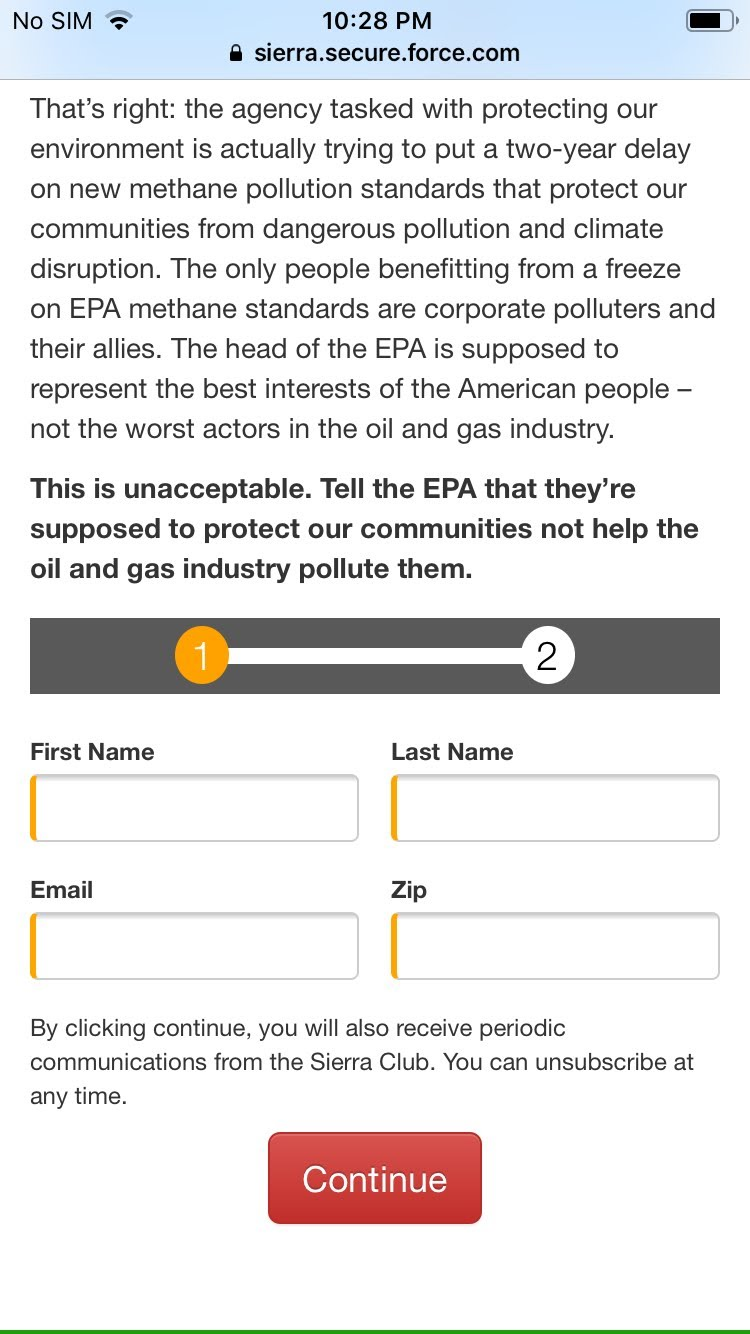
\includegraphics[height = 4in]{Figs/sierra1.jpeg}
    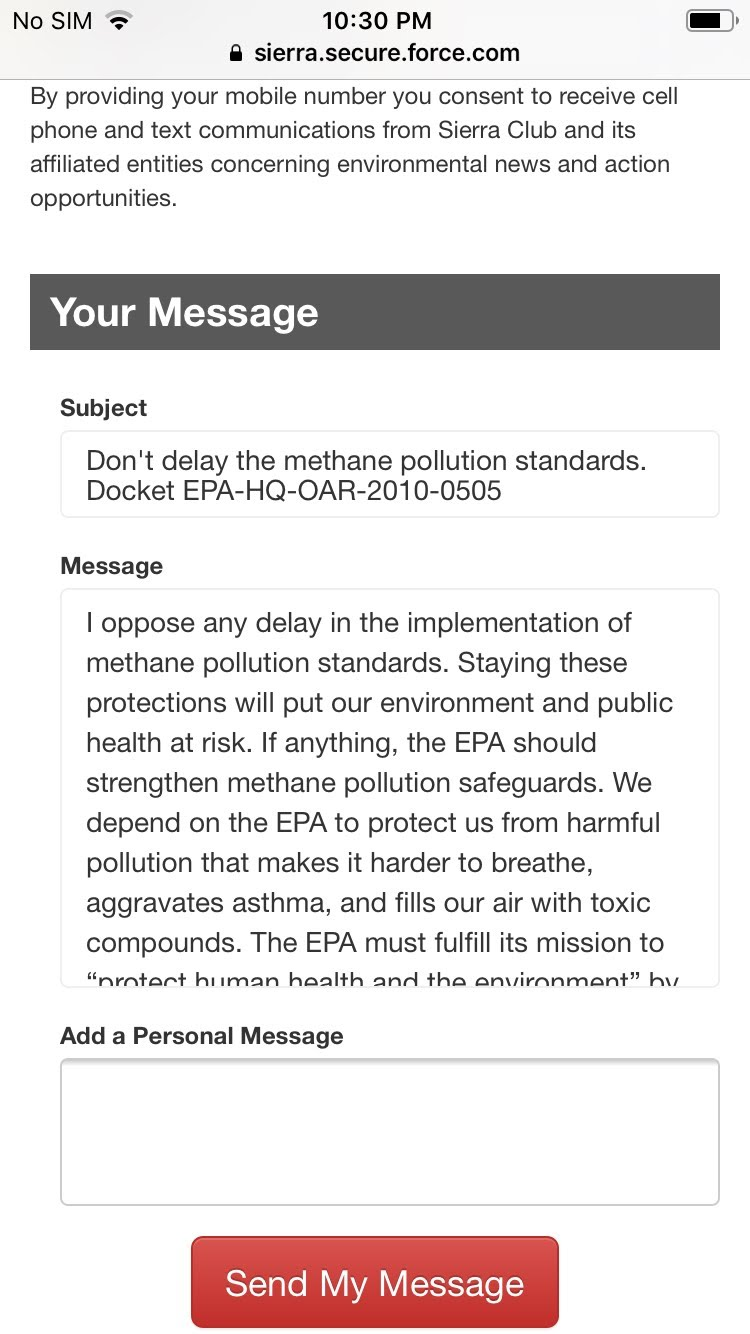
\includegraphics[height = 4in]{Figs/sierra2.jpeg}
    \label{fig:sierra}
\end{figure}

While such campaigns may engage many people, they are unlikely to affect policy or to inspire countermobilization. I expect such campaigns to occur on rules that have high partisan salience (e.g., rules following major legislation passed on a narrow vote), rules that propose large shifts on policy issues dear to member-funded public interest groups, or rulemaking started shortly after presidential transitions when executive-branch agendas shift more quickly than public opinion.

\begin{hyp}
When a lobbying coalition with more intense public support successfully mobilizes for reasons other than influencing policy, opposing coalitions with less public support are not more likely to counter-mobilize.
\end{hyp}

Going public and going down fighting may be difficult to distinguish in the observed public response. Indeed, members of the public may poorly understand the different chances of success in each case. However, lobbying organization do likely know their chances of success and should thus invest less in sophisticated insider lobbying under the going down fighting strategy. By identify cases where coalitions engage in large public campaigns without corresponding investment in sophisticated lobbying, I can assess whether countermobilization and is indeed less likely in these cases. Table \ref{tab:campaigns-patterns} specifies the general pattern of engagement suggested by each of the three reasons behind mass-comment campaigns. 

% CAMPAIGNS-PATTERNS TABLE 
\begin{table}
\small
\centering 
  \caption{Observable differences in engagement across types of mass-mobilization campaigns}
  \def\arraystretch{1.5}
\begin{tabular}{@{\extracolsep{5pt}} lcccc} 
& Inside &  & Outside &   \\ \cline{3-5} 
& Technical information & Number of comments & Effort & Contagion \\
\hline
Going public & High & High & High & High  \\ 
\hline
Disrupting  & High & Low & Low & Low  \\
\hline
Going down fighting & Low & High & High & High  \\ 
\hline 
\end{tabular}
\label{tab:campaigns-patterns}
\end{table}


As Table \ref{tab:campaigns-patterns} suggests, the relevant statistic distinguishing patterns is the \textit{relative} number of each type of comment on each side on a given rulemaking docket. Even among rules targeted by campaigns, salience varies significantly and thus ``high'' and ``low'' numbers of comments will differ across rules. Importantly, even campaigns that achieve very low public response rates appear in these data. Because campaigns aim to collect thousands of comments, it is implausible that even the most unpopular position would achieve no supportive responses. For example, \citet{Potter2017} found Poultry Producers averaging only 319 comments per campaign. While this is far from the Sierra Club's average of 17,325 comments per campaign, it is also far from zero.

% \subsection{Mobilizing for Recruitment}
% A third possibility is that mobilization around bureaucratic decisions is unrelated to the possibility of affecting policy and primarily a way to recruit and engage members or raise the profile of the movement. If this is the case, behaviors like protesting and mass commenting on rules are largely epiphenomena to unrelated kinds of politics. Organizers may know that mobilization has minimal effects, but lead members to engage as a means to other ends. Many of the mobilized themselves may doubt their efficacy but still take advantage of the opportunity to protest. 

\paragraph{Public and private goods.} While coalitions may form around various material and ideological conflicts, those most likely to be advantaged by going public or going down fighting are public interest groups---organizations primarily serving an idea of the public good rather than the material interests of their members.\footnote{\citet{Potter2017} similarly distinguishes ``advocacy groups'' from ``industry groups.'' \citet{Berry1999} calls these groups ``citizen groups'' and emphasizes conflict over cultural issues. While some public interest groups focus on conservative or progressive cultural issues, like religious education, immigration, or endangered species, many are more focused on the public provision or protection of public goods such as national parks, consumer product safety standards, air quality, drinking water, and public safety.

One exception may be types of membership organizations that are both broad and often focused on material outcomes for their members such as labor unions. \citet{Potter2017} puts unions in the ``Industry'' category. I take a different approach based on the coalition with whom such groups lobby. If a union lobbies alongside businesses, I classify this as a private interest-driven coalition. If a union lobbies with public interest groups on public health or safety issues, I classify this as a public interest.} Thus, I theorize that mass mobilization is most likely to occur in conflicts of public versus private interests or public versus public interests (i.e., between coalitions led by groups with distinct cultural ideals or desired public goods), provided they have sufficient resources to run a campaign.
If true, one implication is that mass mobilization will systematically run counter to concentrated business interests where they conflict with the values of public interest groups with sufficient resources to mobilize.


\begin{hyp} \label{hyp:publicinterest}
Public interest group coalitions mobilize more often than business-driven coalitions.
\end{hyp}

Hypothesis \ref{hyp:publicinterest} posits a conditional logic in the decision to mobilize. If resources purely determined outside lobbying, business-driven coalitions would often dominate, as they do elsewhere. However, I argue, because outside lobbying can alter the decision environment, those who have the advantage in the usual rulemaking process (where a more limited set of actors participate) have little incentive to expand the scope of the conflict.




% We do not know who engages in mass commenting. Some assume that people who engage in mass commenting belong to membership organizations. Others imply that they are people who happen to have an opinion. RAUCH discusses both "members" and  _______
% % The people who engage in mass commenting are often assumed to be 

% Engaging a broader audience and thus changing the scope of conflict is a basic political strategy. Presidents, supreme court justices, and others "go public" when doing so alters their opponents' calculations. 

% Which campaigns engage a broader audience and which do not? 


\subsubsection{Types of public engagement} I classify supporters into three types that help describe key pieces of political information. I illustrate these types in the context of public comments. Comments that are exact copies of a form letter are akin to petition signatures from supporters who were engaged by a campaign to comment with minimal effort. Commenters that also take time to add text indicate more intense preferences. Finally, commenters who express solidarity in similar but distinct phrases indicate they were engaged indirectly, perhaps by a news story or a social media post about the campaign, as campaign messages spread beyond those initially targeted.\footnote{It is possible that some people in this latter category engage purely on their own initiative, but any impact they have likely comes from their alignment with a coalition. Furthermore, as I show below, wholly original comments are rare.} Because the success of a mobilization effort is moderated by public support, broader public interest group coalitions ought to mobilize more people, more effort per person, and more people indirectly for the same amount of mobilization effort (e.g., spending or solicitations).  

\begin{hyp}
Public interest group coalitions mobilize more successfully than business-driven coalitions. Indicators of success include (1) the number of comments supporting a coalition (2) the effort per comment (3) the number of comments mobilized indirectly. 
\end{hyp}

\end{subhyp}

The size of each group thus offers political information to policymakers, including coalition resources, the intensity of sentiment, and the potential for conflict to spread. The first two types signal two kinds of intensity or resolve. First, they show the mobilizers' willingness to commit resources to the issue. Second, costly actions show the intensity of opinions among the mobilized segment of the public \citep{Dunleavy1991}. The number of people engaged by a campaign is not strictly proportional to an organization's investment. The less people care, the more it costs to mobilize them. The third type indicates potential contagion. Indications that messages spread beyond those initially targeted may be especially powerful \citep{Kollman1998}. 

Information about organizational resolve, the intensity of public demands, and contagiousness are thus produced, but %, as discussed in section \ref{influence-intro},
such political information will only influence decisions if these signals are processed in a way that captures this information and relays it to decisionmakers. These organizational processes may vary significantly across agencies.

